\documentclass[../main-report.tex]{subfiles}
\begin{document}
\section{Vấn đề đặt ra}
\label{sec:problem}
Trong xã hội công nghệ thông tin đóng vai trò quan trọng hiện nay, tất cả những thông tin cá nhân của chúng ta đều có khả năng bị theo dõi do những hacker xâm nhập và đánh cắp. Đối với một người dùng bình thường, những thông tin đó đôi khi chỉ là những tin nhắn, dòng chat, tài liệu thông thường, nhưng ở mức độ cao hơn điều này gây ra hậu quả vô cùng nghiêm trọng đối với các công ty, tập đoàn do những thông tin mật nếu bị tiết lộ ra ngoài sẽ gây thiệt hại rất lớn. Do đó, nếu như những dữ liệu quan trọng của bạn được bảo mật và mã hóa, sẽ rất khó để hacker có thể theo dõi và đánh cắp được. Việc mã hóa dữ liệu, đơn giản là việc tăng thêm một lớp bảo mật cho dữ liệu bằng cách chuyển đổi dữ liệu sang một dạng khác thông qua một mã khóa với những quy tắc tùy biến. Vì vậy, kể cả khi dữ liệu của bạn có bị đánh cắp, việc giải mã dữ liệu cũng là rất khó khăn. Một ví dụ đơn giản cho việc mã hóa dữ liệu: Nếu như bạn chỉ đặt mật khẩu cho máy tính, laptop của bạn, hacker chỉ cần một vài thủ thuật để bỏ qua lớp mật khẩu là có thể truy cập được dữ liệu, hoặc đơn giản chỉ là cắm thiết bị lưu trữ sang một hệ thống khác, tuy nhiên nếu như dữ liệu được mã hóa, kể cả khi có được dữ liệu rồi cũng rất khó để giải mã được như ban đầu nếu không có mã khóa.

Ngày nay với sự ra đời của thế giới kỹ thuật số, việc giao tiếp của con người đã trở thành một trong những khía cạnh thiết yếu nhất của cuộc sống, dễ dàng và nhanh chóng hơn. Ta có thể dễ dàng thực hiện giao tiếp thời gian thực với bạn bè và gia đình ở bất kỳ nơi nào trên thế giới thông qua các ứng dụng trò chuyện, email và các công cụ dựa trên web phổ biến khác. Ngày càng có nhiều người sử dụng các ứng dụng điện thoại thông minh để trò chuyện, và theo đó, nguy cơ nội dung tin nhắn bị tin tặc nghe lén càng tăng cao. Nếu chỉ sử dụng mã hóa khi truyền tải không thì sẽ rất nguy hiểm khi mà nội dung trò truyện có thể rò rỉ nếu server bị hacker xâm nhập do dữ liệu chỉ mã hóa trên đường truyền chứ không mã hóa khi lưu vào cơ sở dữ liệu. Do đó, Facebook, Whatsapp, Viber hay các nền tảng nhắn tin khác đã và đang áp dụng phương thức mã hóa End-to-end Encryption (E2EE) trong ứng dụng của họ. E2EE là phương thức mã hóa mà chỉ duy nhất những người giao tiếp với nhau có thể hiểu được thông điệp được mã hóa. Điều này đồng nghĩa với việc kể cả chủ sở hữu của kênh truyền tải dữ liệu, những nhà cung cấp dịch vụ Internet hay hacker cũng khó có thể biết được những thông tin người giao tiếp đang truyền tải. Phương thức mã hóa này sử dụng mã khóa (key) thuộc về những người đang trực tiếp liên lạc và truyền tải thông tin, dữ liệu, và nếu không có mã khóa này, không một bên thứ ba nào có thể giải mã dữ liệu.


\begin{figure}[ht!]
\begin{center}
\label{fig:E2E}
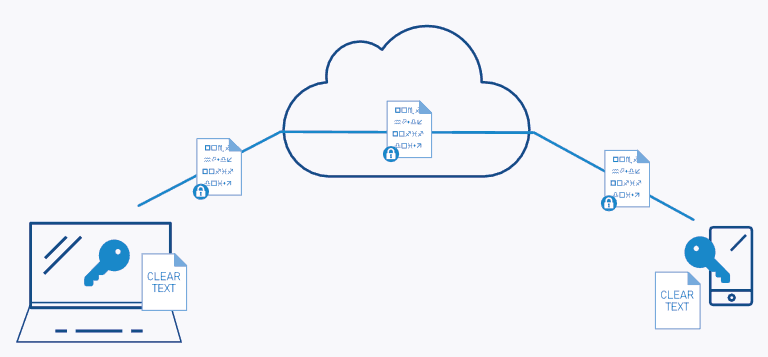
\includegraphics[scale=0.65]{E2E}
\caption{Mô hình mã hóa end to end encryption}
\end{center}
\end{figure}

Khi thế giới chuyển sang mã hóa đầu cuối cho các nền tảng nhắn tin cá nhân, các doanh nghiệp cũng đang tích hợp chúng mức độ bảo mật trong các ứng dụng nhắn tin của công ty. Giao thức Signal [\cite{1}], được triển khai cho cơ sở một tỷ người dùng của WhatsApp vào năm 2016, là giao thức mã hóa đầu cuối đầu tiên được triển khai trên toàn cầu. Đây là một giao thức mật mã không liên kết, có thể được sử dụng để cung cấp mã hóa đầu cuối cho các cuộc gọi thoại, cuộc gọi video và các cuộc hội thoại nhắn tin tức thời. Signal với tiêu chí hoạt động là đảm bảo tính riêng tư tối đa cho người dùng, dịch vụ này không lưu trữ bất kì dữ liệu gì của khách hàng, kể cả dữ liệu đã mã hóa. Ngoài ra còn có các giao thức như Secure Real-time Transport Protocol (SRTP) [\cite{2}], Elliptic-curve Diffie–Hellman [3], ZRTP (gồm Z và Real-time transport Protocol)… cũng là các giao thức cung cấp mã hóa đầu cuối, thành lập kênh trò chuyện bí mật thông qua phương pháp trao đổi khóa Diffie–Hellman.

SRTP là cấu hình giao thức Real-time Transport Protocol, nhằm cung cấp mã hóa, xác thực và tính toàn vẹn của tin nhắn và bảo vệ dữ liệu RTP khỏi replay attack trong cả ứng dụng unicast và multicast. Nó được phát triễn bởi một nhóm nhỏ các Internet Protocol và các chuyên gia mật mã từ Cisco và Ericsson.


\begin{figure}[ht!]
\begin{center}
\label{fig:SRTP}
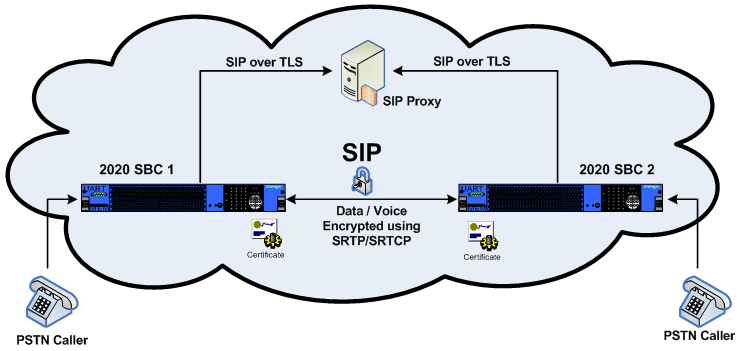
\includegraphics[scale=0.7]{SRTP}
\caption{Secure Real-time Transport Protocol (SRTP)}
\end{center}
\end{figure}

ZRTP là một giao thức trao đổi khóa mật mã để đàm phán các khóa để mã hóa giữa hai điểm cuối trong cuộc gọi điện thoại thông qua Voice over Internet Protocol (VoIP) dựa trên giao thức Real-time Transport Protocol. Nó sử dụng trao đổi khóa của Diffie-Hellman và giao thức SRTP để mã hóa.

\begin{figure}[ht!]
\begin{center}
\label{fig:ZRTP}
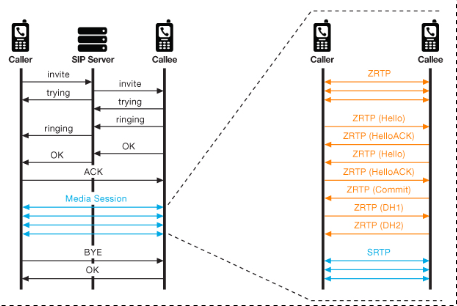
\includegraphics[scale=0.85]{ZRTP}
\caption{ZRTP (gồm Z và Real-time transport Protocol)}
\end{center}
\end{figure}

Các giao thức trên đều có ưu và nhược điểm riêng, tuy nhiên, chúng đều có chung một nhược điểm là đều cung cấp một giao thức thỏa thuận khóa bí mật để mã hóa thông tin chỉ giữa hai điểm đầu cuối. Tức là mã hóa đầu cuối hiện tại chỉ hỗ trợ trao đổi thông tin giữa hai người duy nhất và không hỗ trợ khi có thêm người thứ ba. Điều này là đúng với các ứng dụng phổ biến hiện nay như Viber, Telegram, hay thậm chí là Facebook Messenger. Các ứng dụng nói trên đều hỗ trợ trò chuyện riêng tư thông qua mã hóa đầu cuối, nhưng chỉ hỗ trợ giữa hai thành viên với nhau. Wire [4], một ứng dụng hiếm hoi ít người biết đến, là ứng dụng hiện tại có hỗ trợ mã hóa đầu cuối cho việc trao đổi thông tin nhóm. Tuy nhiên, thực tế cho thấy cốt lõi của việc mã hóa đầu cuối trong nhóm mà Wire sử dụng vẫn chỉ là mã hóa giữa hai người với nhau [5]. 
	
Để giải quyết khó khăn trên, Lực lượng Chuyên trách về Kỹ thuật Liên mạng (IETF) đã và đang xây dựng lên giao thức Messaging Layer Security (MLS) [6] – một chuẩn giao thức chung hiện đại, an toàn bảo mật cho việc nhắn tin nhóm. MLS là một lớp bảo mật để mã hóa tin nhắn trong nhóm có số lượng thành viên lớn. Mục đích MLS hướng tới xây dựng một chuẩn giao thức chung, có thể ứng dụng đa nền tảng, hỗ trợ mã hóa tin nhắn trong nhóm chứa đến 50000 thành viên và đảm bảo an ninh bảo mật thông tin. Đáp ứng đầy đủ yêu cầu bảo mật như: Forward Secrecy (FS) – Trong mật mã còn được gọi là Perfect Forward Secrecy (FFS), là một tính năng của giao thức thỏa thuận khóa cụ thể mang lại sự đảm bảo rằng các khóa phiên sẽ không bị xâm phạm ngay cả khi khóa riêng của máy chủ bị xâm phạm. Post-compromise security (PCS) – Kể từ khi khóa riêng của máy chủ bị xâm phạm vẫn đảm bảo rằng các khóa phiên của người dùng trong tương lai sẽ không bị xâm phạm.

\begin{figure}[ht!]
\begin{center}
\label{fig:MLS-base}
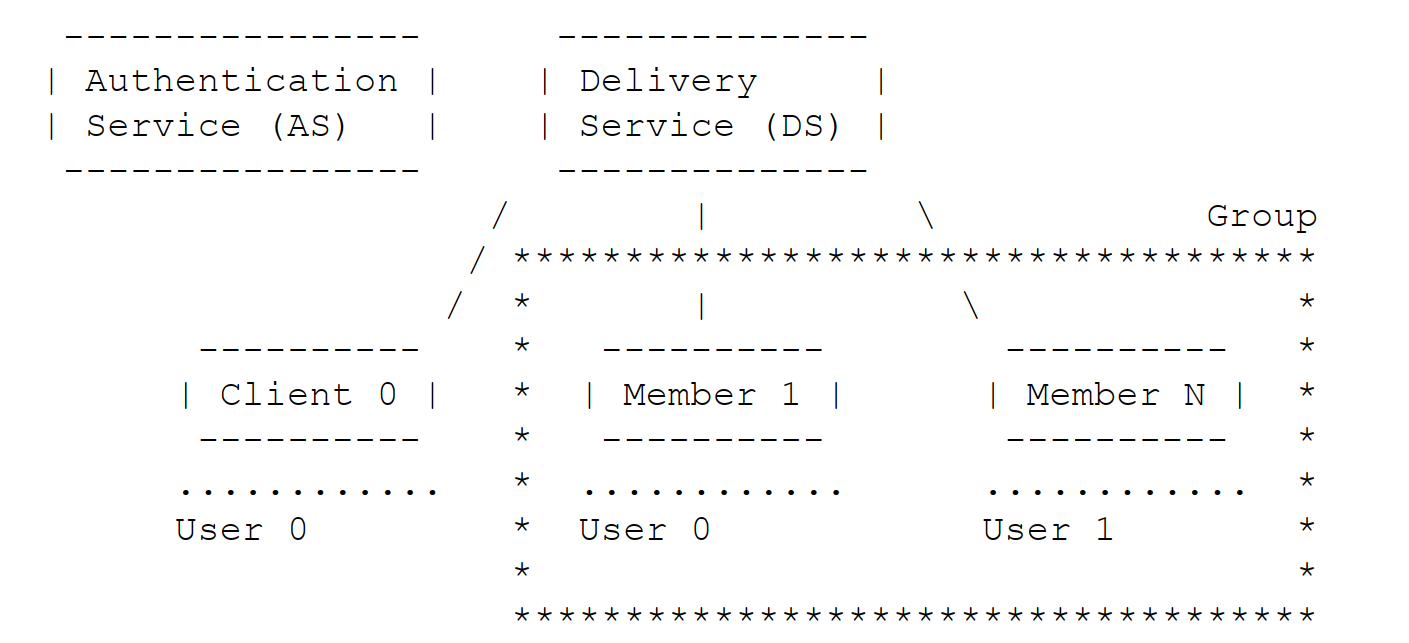
\includegraphics[scale=0.5]{MLS-base}
\caption{Mô hình kiến trúc cơ bản của giao thức MLS}
\end{center}
\end{figure}

Xuất phát từ hạn chế trên và từ lợi ích có được khi sử dụng giao thức MLS, đề tài này hướng tới việc tạo nên một kênh giao tiếp bí mật, truyền tải thông tin nhạy cảm một cách riêng tư và chỉ có người liên quan mới có thể đọc được. Kết quả của nghiên cứu này sẽ nâng cao tính an toàn, bảo mật cho dữ liệu, tránh những trường hợp thất thoát thông tin dữ liệu quan trọng khi giao tiếp thông qua internet. 


\section{Tính khoa học và tính mới của đề tài}
\subsection{Tính khoa học}

Nghiên cứu này sẽ tập trung nghiên cứu vấn đề mã hóa đầu cuối trong khi nhắn tin nhóm dựa trên MLS protocol. Nghiên cứu chi tiết cách hoạt động và triển khai giao thức MLS. Nghiên cứu cơ chế hoạt động của các thuật toán mã hóa đầu cuối, kết hợp các thuật toán vào xây dựng một ứng dụng nhắn tin nhóm đáp ứng yêu cầu số lượng thành viên lớn và đạt hiệu suất cao.

Đề tài này hướng đến việc xây dựng ứng dụng nhắn tin nhóm an toàn, riêng tư, bí mật. Ứng dụng này có các chức năng cơ bản cho việc nhắn tin bí mật giữa nhiều thành viên trong nhóm với nhau, đảm bảo tính riêng tư, bí mật thông qua áp dụng mã hóa đầu cuối, đáp ứng nhu cầu trao đổi thông tin nhạy cảm cho công ty, doanh nghiệp có số lượng nhân viên lớn. Nếu nghiên cứu thành công, thì đây sẽ là ứng dụng đầu tiên áp dụng mã hóa đầu cuối vào việc trao đổi thông tin giữa nhiều cá nhân, đáp ứng nhu cầu bảo đảm bí mật thông tin trao đổi khỏi bị theo dõi hay bị đánh cắp cho các công ty, doanh nghiệp.


\subsection{Tính mới}

Trên thế giới, số công trình nghiên cứu ứng dụng hỗ mã hóa đầu cuối vào việc trao đổi thông tin trong nhóm ở thực tiễn hầu như không có hoặc đang nghiên cứu nhưng không công khai. Từ đó, vấn đề nghiên cứu này sẽ đáp ứng nhu cầu nhắn tin nhóm cho các doanh nghiệp có yêu cầu cao trong việc bảo vệ sự riêng tự, bí mật, an toàn. 

\section{Mục tiêu}

Xây dựng ứng dụng nhắn tin nhóm cơ bản dựa trên MLS protocol có các thuộc tính cơ bản như trên. 
Ứng dụng có các chức năng chính:

\begin{itemize}
\item Tạo nhóm.
\item Xóa nhóm.
\item Thêm người dùng vào nhóm.
\item Xóa người dùng khỏi nhóm.
\end{itemize}

\section{Đối tượng nghiên cứu}
\begin{itemize}
\item Giao thức MLS.
\item Các thuật toán liên quan đến mã hóa đầu cuối như SRTP, ZRTP,…
\end{itemize}

\section{Phạm vi nghiên cứu}
Ứng dụng có các chức năng cơ bản cho việc trao đổi thông tin bằng văn bản.
\end{document}